\documentclass[11pt,oneside,a4paper]{article}
\usepackage[utf8]{inputenc}
\usepackage[spanish]{babel}
\usepackage{multirow} 
\usepackage{graphicx}
\graphicspath{{images}}
\title{Memoria práctica 2}
\author{Marcos Esteve Casademunt, Jose Gómez Gadea}
\usepackage{listings}

\date{Noviembre 2017}

\makeindex

\begin{document}

\maketitle
\tableofcontents
\newpage
\section{Descripción del problema}
Se desea calcular la cantidad de divisores exactos que tienen cada uno de los M primeros números naturales, con la intención de mostrar los N números enteros dentro de ese rango que tienen una mayor cantidad de divisores.
\section{Definiciones}
\begin{itemize}

\item \textbf{Speed-up} indica la ganancia de velocidad que consigue el
algoritmo paralelo con respecto a un algoritmo secuencial.
\begin{equation}
S(n,p) =  \frac{t(n)}{ t(n,p)}
\end{equation}
\item \textbf{Eficiencia} mide el grado de aprovechamiento que un algoritmo paralelo hace de un computador paralelo.
\begin{equation}
E(n,p) = \frac{S(n,p)}{p}
\end{equation}

\end{itemize}
\section{Ejercicios}
Una vez presentadas las definiciones básicas, pasamos a analizar los resultados de la práctica:
\subsection{Ejercicio 1}
En este ejercicio se pretende medir el tiempo del bucle principal, para ello hemos añadido las siguientes lineas.
\lstset{language=C, breaklines=true, basicstyle=\footnotesize}
\begin{lstlisting}[frame=single,  showstringspaces=false]
t0 = omp_get_wtime();
  for ( n = 1 ; n <= M ; n++ ) {
   ...
  }
t1 = omp_get_wtime();
printf("Tiempo: %f s", t1-t0);
\end{lstlisting}
\subsection{Ejercicio 2}
En este ejercicio se pretende analizar si son paralelizables los tres bucles así como calcular las prestaciones.
\subsubsection{Primer bucle}
El primer bucle si se puede paralelizar. Para ello debemos hacer privadas las variables c, i, ini, inc que son independientes para cada iteración. Además será necesario usar una sección crítica  ya que dos iteraciones distintas pueden escribir en el mismo valor del array.
\lstset{language=C, breaklines=true, basicstyle=\footnotesize}
\begin{lstlisting}[frame=single]

#pragma omp for private(c,i,ini, inc)
  for ( n = 1 ; n <= M ; n++ ) {
    c = 1; /* por el 1, que siempre es divisor */
    ...
    ...
    
    if ( MEJOR(n,c,N-1) ) {
      #pragma omp critical
        if ( MEJOR(n,c,N-1) ) {
        for ( i = N - 1 ; i > 0 && MEJOR(n,c,i-1) ; i-- ) {
          vc[i] = vc[i-1]; vn[i] = vn[i-1];
        }
        vc[i] = c; vn[i] = n;
      }
    }
  }
\end{lstlisting}
Pasamos por tanto a analizar los tiempos de esta paralelización:


\begin{table}[htbp]
\begin{center}
\begin{tabular}{|l|l||l|l||l||l|}
\hline
Planificación & 2 & 4 & 8 & 16 & 32 \\
\hline 
Static 0 & 26.098569 & 15.369443 & 8.308206 & 4.834699 & 3.126337\\\hline
Static 1 & 22.969833 & 11.502033 & 6.292179 & 3.592557 & 2.471968 \\\hline
Static 2 & 17.304959 & 8.623851 & 5.019181 & 2.696642 & 1.853828 \\ \hline
Dynamic 1 & 17.251117 & 8.627753 & 4.496865 & 2.693916 & 1.849314 \\ \hline
Dynamic 2 & 17.234738 & 8.622996 & 4.586967 & 2.693860 & 1.849164 \\ \hline
\end{tabular}
\caption{Tiempos de ejecución}
\label{tabla:tiempos}
\end{center}
\end{table}
Como podemos observar, una planificación dinámica reduce el tiempo de ejecución del programa. Esto se puede apreciar mejor en la gráfica mostrada a continuación. 
\begin{center}
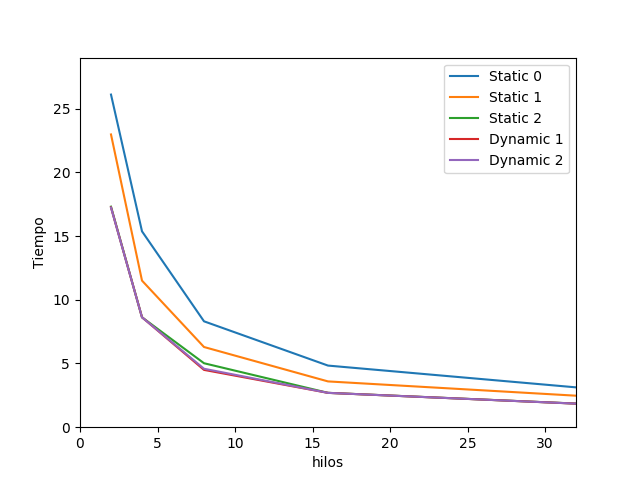
\includegraphics[scale=0.7]{/tiempo.png}
\end{center}
En cuanto al Speed-up (Tiempo secuencial aproximadamente 34.55s) 
\begin{table}[htbp]
\begin{center}
\begin{tabular}{|l|l||l|l||l||l|}
\hline
Planificación & 2 & 4 & 8 & 16 & 32 \\\hline 
Static 0 & 1.32 &2.24 &4.15 &7.15 &11.07\\\hline
Static 1 & 1.50 &3&5.48&9.62&13.98\\\hline
Static 2 &  1.99 &4&6.88&12.84&18.67 \\ \hline
Dynamic 1 &2 &4&7.694&12.84&18.67 \\ \hline
Dynamic 2 &2.02 &4&7.54&12.84&18.67\\ \hline
\end{tabular}
\caption{Speed-Up}
\label{tabla:speedup}
\end{center}
\end{table}

Las planificaciones Dynamic junto con static con chunck 2 obtienen mejores Speed-Ups en comparación con el resto de planificaciones. Esto se puede observar en la siguiente gráfica.
\begin{center}
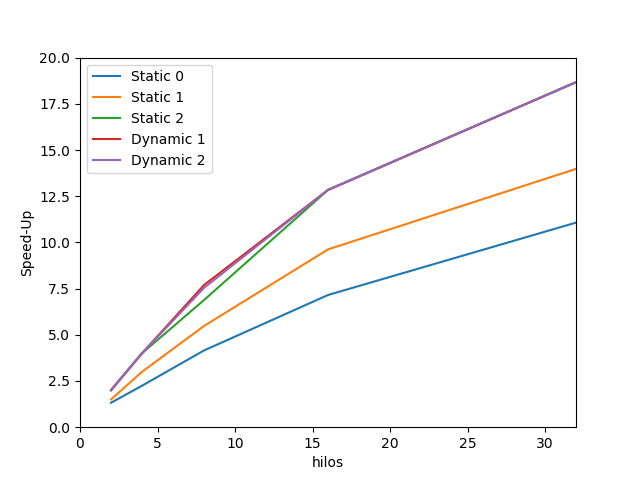
\includegraphics[scale=0.7]{/speedup.png}
\end{center}

Por último analizando la eficiencia...
\begin{table}[htbp]
\begin{center}
\begin{tabular}{|l|l||l|l||l||l|}
\hline
Planificación & 2 & 4 & 8 & 16 & 32 \\\hline 
Static 0 &  0.660 &0.561&0.519&0.447&0.345\\\hline
Static 1 & 0.751 &0.75&0.685&0.601&0.436 \\\hline
Static 2 &  0.996 &1&0.86&0.802&0.583 \\ \hline
Dynamic 1 & 1 &1&0.961&0.802&0.583 \\ \hline
Dynamic 2 &  1 &1 &0.942&0.802&0.583 \\ \hline
\end{tabular}
\caption{Eficiencia}
\label{tabla:eficiencia}
\end{center}
\end{table}

Como podemos observar, la máquina paralela está mejor aprovechada con  2, 4 hilos y con las planificaciones Static con chunck 2 y Dynamic. Esto se puede observar mejor en la siguiente gráfica.

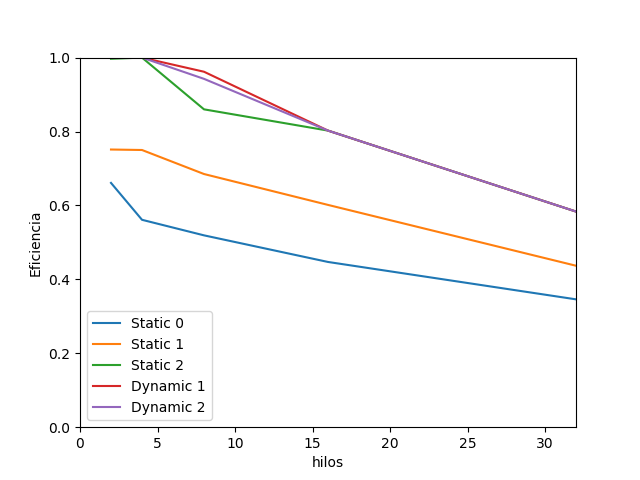
\includegraphics[scale=0.7]{/eficiencia.png}

\subsubsection{Segundo bucle}
El segundo bucle si se puede paralelizar. Para ello debemos hacer una reducción sumando de c. 
\lstset{language=C, breaklines=true, basicstyle=\footnotesize}
\begin{lstlisting}[frame=single]
#pragma omp parallel for reduction(+:c)
for ( i = ini ; i <= n ; i += inc ) {
      if ( n % i == 0 ) c++;
}
\end{lstlisting}

Pasamos a analizar los tiempos de ejecución al paralelizar este segundo bucle:
\begin{table}[htbp]
\begin{center}
\begin{tabular}{|l|l||l|l||l||l|}
\hline
Planificación & 2 & 4 & 8 & 16 & 32 \\
\hline 
Static 0 & 20.530381 &10.729977 &6.503967 &5.394774 &5.210012\\\hline
Static 1 & 65.497120 &41.851255 &24.181914&13.017211&10.364424 \\\hline
Static 2 & 42.421072 &26.000943 &14.932108 &10.405176 &8.495147 \\ \hline
Dynamic 1 & 523.593595 &394.736502 &337.955795 &476.433302 &600.608951 \\ \hline
Dynamic 2 & 140.707958 &182.115155 &185.497058 &281.455687 &318.156567  \\ \hline
\end{tabular}
\caption{Tiempos de ejecución}
\label{tabla:tiempos2}
\end{center}
\end{table}

Como podemos observar, los tiempos con planificaciones dinámicas son significativamente mayores que los tiempos con planificaciones estáticas. Esto es debido a que las planificaciones dinámicas tienen un sobre coste mayor por cada proceso respecto a las planificaciones estáticas pese a que tienen una mejor paralelización (y por tanto, salvo excepciones como esta, suelen dar mejor resultado). Además, esta segunda paralelización será más ineficiente que la paralelización del primer bucle ya que los hilos se activarán y desactivarán tantas veces como iteraciones haga el bucle principal, y esto hará que el sobre coste repercuta demasiado en el tiempo de ejecución. Algunas de estas conclusiones se pueden observar visualmente en la siguiente gráfica.

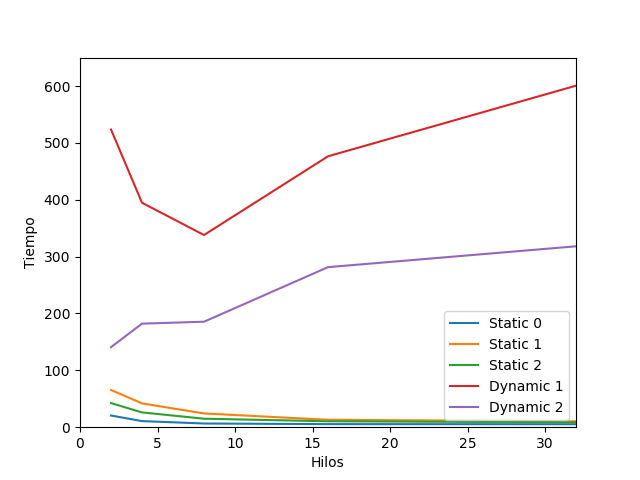
\includegraphics[scale=0.7]{/tiempo2.png}

En cuanto al Speed-up:

\begin{table}[htbp]
\begin{center}
\begin{tabular}{|l|l||l|l||l||l|}
\hline
Planificación & 2 & 4 & 8 & 16 & 32 \\
\hline 
Static 0 & 1.68 &3.21 &5.3 &6.4 &6.62 \\\hline
Static 1 & 0.52 &0.82 &1.42 &2.65 &3.33  \\\hline
Static 2 & 0.81 &1.32 &2.31 &3.31 &4.06 \\ \hline
Dynamic 1 & 0.0658 &0.087 &0.1 &0.07 &0.0575 \\ \hline
Dynamic 2 & 0.24 &0.18 &0.18 &0.12 &0.10  \\ \hline
\end{tabular}
\caption{Speed-Up}
\label{tabla:speed2}
\end{center}
\end{table}
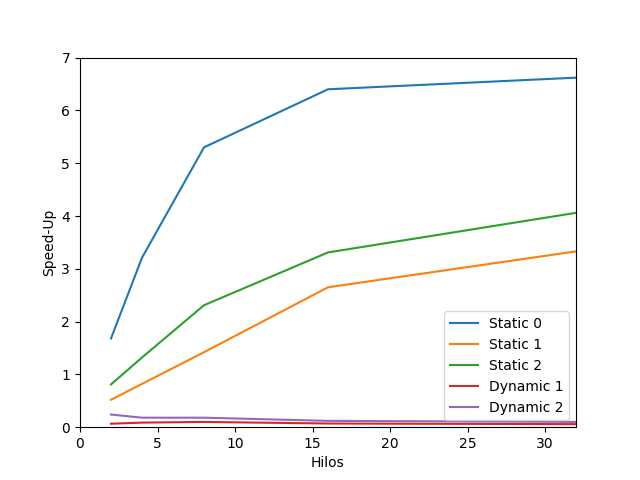
\includegraphics[scale=0.7]{/speedup2.png}

Por último, analizando la eficiencia...
\begin{table}[htbp]
\begin{center}
\begin{tabular}{|l|l||l|l||l||l|}
\hline
Planificación & 2 & 4 & 8 & 16 & 32 \\
\hline 
Static 0 & 0.84 &0.80 &0.6625 &0.4 &0.206\\\hline
Static 1 & 0.26 &0.205 &0.177 &0.165 &0.10  \\\hline
Static 2 & 0.405 &0.33 &0.288 &0,20 &0.12  \\ \hline
Dynamic 1 & 0.0329 &0.021 &0.125 &0.0043 &0.0017  \\ \hline
Dynamic 2 & 0.12 & 0.045 &0.02 & 0.0075 &0.0031 \\ \hline
\end{tabular}
\caption{Eficiencia}
\label{tabla:eficiencia2}
\end{center}
\end{table}

\includegraphics[scale=0.7]{/eficiencia2.png}
\subsubsection{Tercer bucle}

El tercer bucle no se puede paralelizar. Esto es debido a que existe una dependencia entre sus iteraciones ya que, en la iteración i, se lee el valor de la iteración i-1. 
\lstset{language=C, breaklines=true, basicstyle=\footnotesize}
\begin{lstlisting}[frame=single]
for ( i = N - 1 ; i > 0 && MEJOR(n,c,i-1) ; i-- ) {
	vc[i] = vc[i-1]; vn[i] = vn[i-1];
}
\end{lstlisting}
\subsection{Ejercicio 3}
En este ejercicio se pretende  que cada hilo muestre la cantidad total de divisores. Para ello, creamos una variable privada para toda la región paralela. Además, en el bucle de contar divisores incrementamos la variable y por último mostramos por cada hilo la cantidad de divisores que ha calculado.


\lstset{language=C, breaklines=true, basicstyle=\footnotesize}
\begin{lstlisting}[frame=single , showstringspaces=false]
int nDiv = 0;
  #pragma omp parallel private(nDiv)
  {
    #pragma omp for private(c, ini, inc, i)
    for ( n = 1 ; n <= M ; n++ ) {
     ...
     ...
      /* Contar divisores */
      for ( i = ini ; i <= n ; i += inc ) {
        if ( n % i == 0 ) {
          c++;
          nDiv++;
        }
      }
      if ( MEJOR(n,c,N-1) ) {
        #pragma omp critical
        {
         ...
         ...
      }
    }
    printf("Hilo %d: %d divisores.\n",omp_get_thread_num(),nDiv);
  }
\end{lstlisting}

\subsection{Ejercicio 4}
En este último ejercicio se pretende paralelizar de forma manual el bucle que funcione mejor(el más externo en nuestro caso).
La parelización será idéntica al primer bucle, pero cambiando el parallel for por lo siguiente:
\lstset{language=C, breaklines=true, basicstyle=\footnotesize}
\begin{lstlisting}[frame=single, showstringspaces=false]
#pragma parallel  private(c, i, ini, inc, yo)
  {
    yo = omp_get_thread_num();
    numhilos = omp_get_num_threads();
    for ( n = yo +1; n <= M ; n+=numhilos ) {
     ...
     ...
     ...
      if ( MEJOR(n,c,N-1) ) {
        #pragma omp critical
       
          if ( MEJOR(n,c,N-1) ) {
          for ( i = N - 1 ; i > 0 && MEJOR(n,c,i-1) ; i-- ) {
            vc[i] = vc[i-1]; vn[i] = vn[i-1];
          }
          vc[i] = c; vn[i] = n;
        }
      }
    }
}
}
\end{lstlisting}
 

\section{Conclusiones}
Como conclusiones, nos gustaría recalcar:
\begin{itemize}
\item 
Como se ha podido observar, paralelizar el bucle más externo es más eficiente que paralelizar el bucle interno. Esto es debido a que  paralelizar el bucle interno añade al tiempo un sobrecoste de activación y desactivación de los hilos. 
\item También se ha podido observar que en este caso las planificaciones Dynamic y Static con chunk 2 obtienen mejores tiempos que las demás planificaciones. Esto es debido  a que  todas las iteraciones no tienen la misma carga y por tanto, un reparto dinámico repartirá mejor la carga entre los distintos hilos.
\item Por último, nos gustaría destacar que esta práctica nos ha ayudado a confirmar algunos conocimientos explicados en teoría (medida  de prestaciones, planificaciones estáticas y dinámicas... ). 
\end{itemize}

\end{document}
